\chapter{Analýza požadavků}
 \label{chap:specification}
Analýza požadavků je prvotní fáze návrhu softwaru a zaměřuje se na sběr požadavků, jejich pochopení a formalizaci. Dále zde může být zahrnuta studie proveditelnosti, formalizace požadavků a akceptační testování. Prvotní požadavky jsou často sbírány analýzou stávajícího řešení nebo řízeným rozhovorem se zadavatelem. V mém případě se jedná o analýzu stávajících řešení, kterou jsem provedl v rámci kapitoly \ref{chap:archives} Webové aplikace pro zpřístupnění digitalizovaných archiválií. 

\section{Diagram případů užití}
Diagram případů užití \cite{useCase} je UML diagram chování zachycující funkcionalitu systému a~aktéry, kteří v~rámci systému mohou vystupovat. Z diagramu je dále patrný rozsah implementovaného systému. V~tomto systému vystupuje pouze role uživatele, jenž v~případě, že je přihlášen, má vyšší práva a~může provádět více operací jako například přidávat poznámky a záložky k jednotlivých archivním skenům.
\begin{figure}[htbp]
\centering
    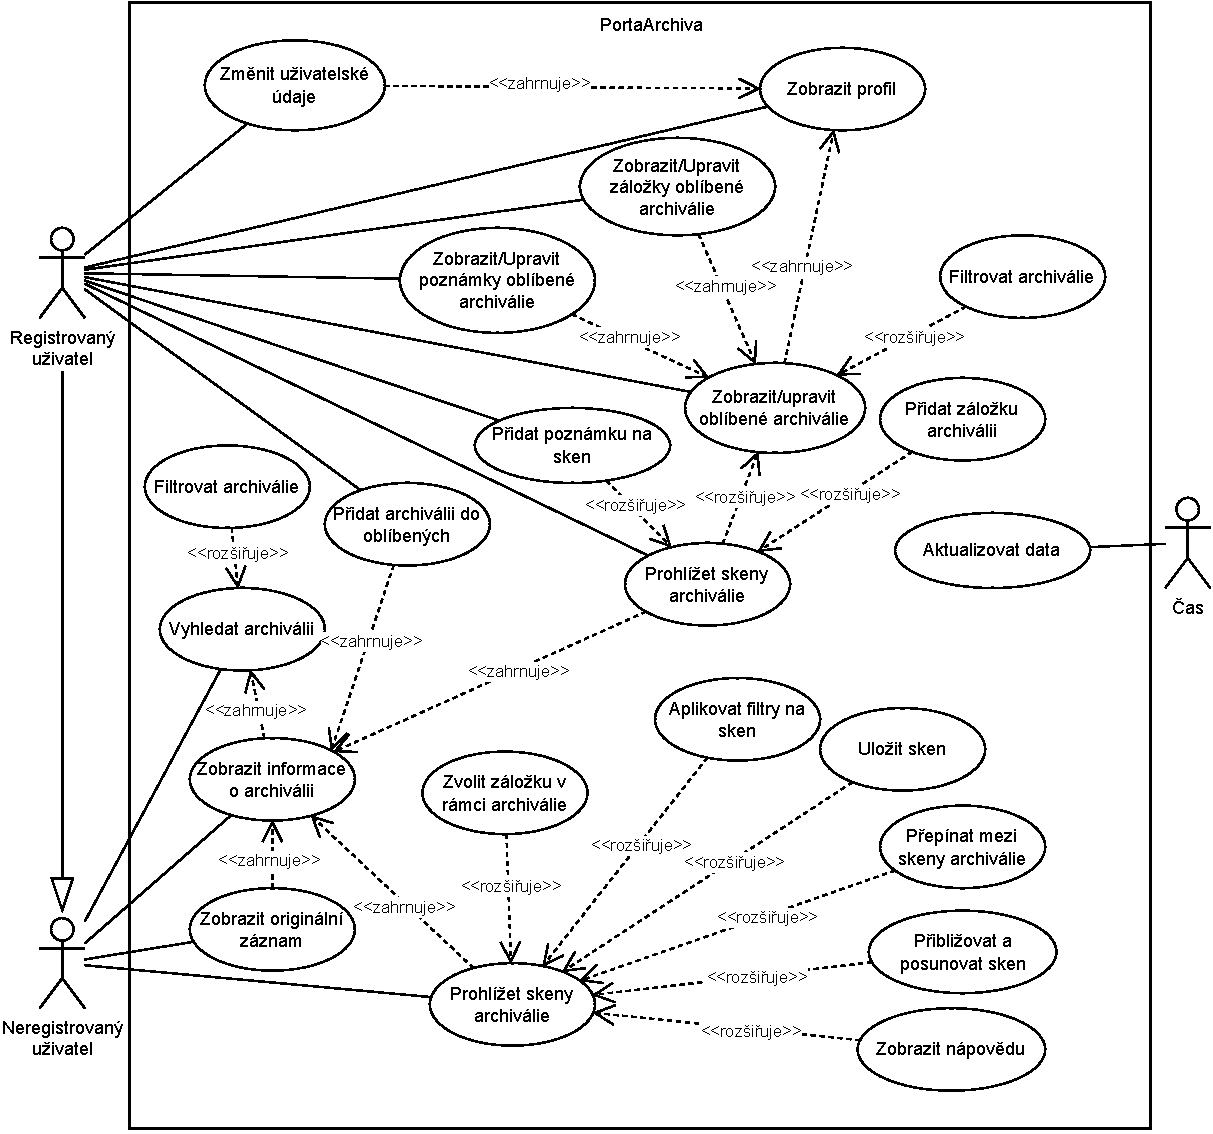
\includegraphics[scale=.75]{obrazky-figures/specification/useCase.pdf}
    \caption{Diagram případů užití}
\end{figure}

\newpage
\section{Systémové diagramy sekvence}
Systémový diagram sekvence \cite{systemSequenceDiagram} slouží pro vizualizaci sledu interakcí uživatele se systémem. Jeho hlavním cílem je detailněji popsat a~znázornit jednotlivé kroky, které uživatel vykonává při práci se systémem.
\newpara
První diagram znázorňuje průchod systémem a~vyhledání konkrétní archiválie v~dané kategorii po specifikování filtrů. Při zobrazení detailu archiválie může přihlášený uživatel přidat danou archiválii do oblíbených. Dále si uživatel může zobrazit prohlížeč skenů nebo záznam na stránkách zdrojového archivního webu.
\begin{figure}[htbp]
\centering
    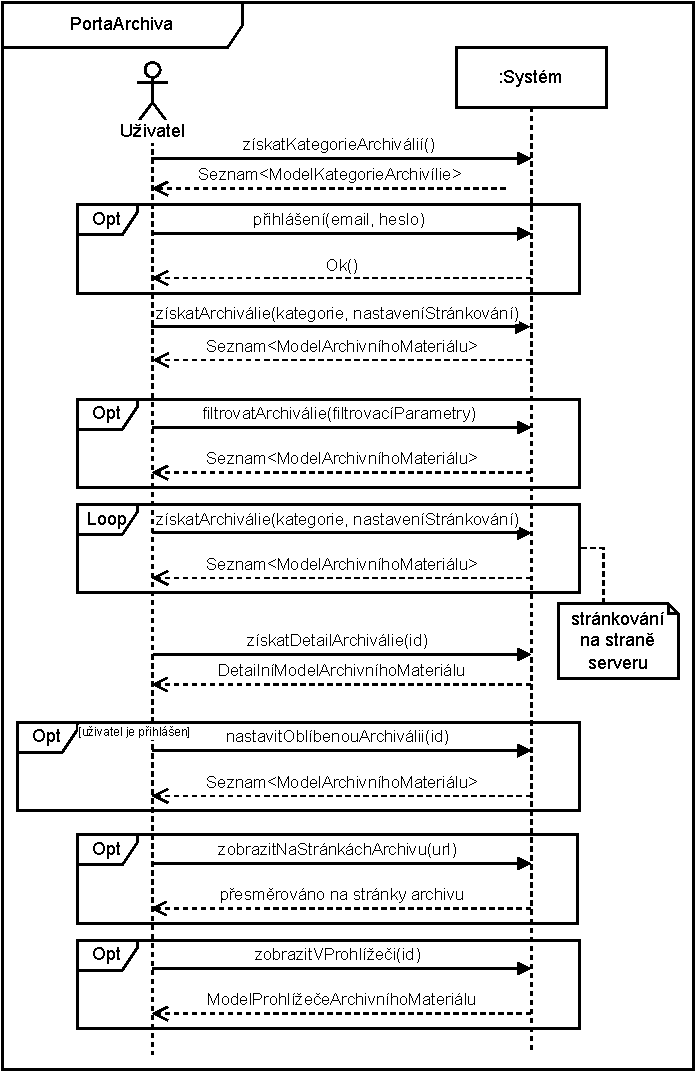
\includegraphics[scale=.8]{obrazky-figures/specification/SSD_find_archival_material.pdf}
    \caption{Systémové diagramy sekvence – vyhledání archiválie}
\end{figure}

\newpage
\noindent Další diagram se zaměřuje na prohlížení archiválie, jelikož se jedná o primární funkcionalitu. Uživatel si může zobrazit nápovědu, upravit kontrast nebo jas pomocí filtrů a~nastavit režim celé obrazovky. Následně už se opakovaně pohybuje po archiválii a~přepíná mezi jednotlivými naskenovanými folii archiválie.

\begin{figure}[htbp]
\centering
    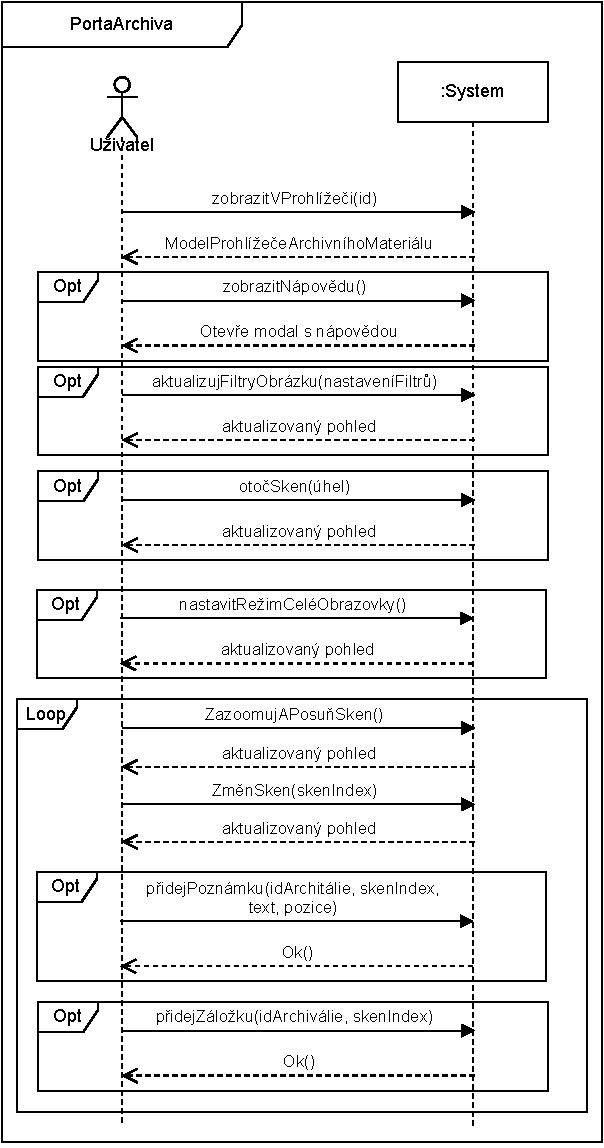
\includegraphics[scale=.85]{obrazky-figures/specification/SSD_preview_scans.pdf}
    \caption{Systémové diagramy sekvence - prohlížení archiválie}
\end{figure}

\newpage
\noindent
Poslední systémový diagram sekvence se zaměřuje na uživatelský profil, kde byla pro jednoduchost modelována práce pouze s~oblíbenými matrikami. Uživatel může odebrat oblíbenou matriku a~obdobně jako u detailního pohledu může přejít na stránky archivu, který danou archiválii zveřejnil, nebo do prohlížeče archiválií. V~rámci profilu je dále možné zobrazit a~editovat jednotlivé záložky nebo poznámky vytvořené daným uživatelem.

\begin{figure}[htbp]
\centering
    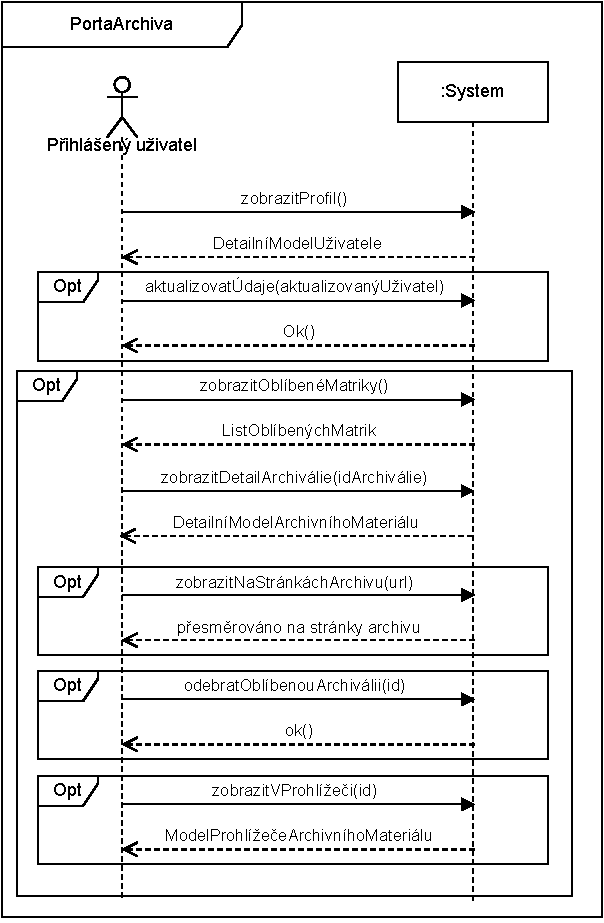
\includegraphics[scale=.9]{obrazky-figures/specification/SSD_user_profile.pdf}
    \caption{Systémové diagramy sekvence – uživatelský profil}
\end{figure}

\newpage
\section{Doménový model}
Doménový model \cite{domainModel} se tvoří v~rané fázi vývoje a~slouží pro identifikaci entit, jež se v~dané doméně vyskytují. Dále je potřeba určit jednotlivé vazby mezi entitami. Každá vazba má kardinalitu, kolikrát daná entita může vystupovat v~konkrétním vztahu (například jeden bankovní účet má právě jednoho vlastníka, ale může mít více disponentů). V~rámci doménového modelu se nutně nemusí vyskytovat datové typy. V~případě, že jsou datové typy uváděny, tak by neměly být závislé na konkrétní technologii. V~době tvorby tohoto modelu se pouze zkoumá, zda se jedná o~textovou hodnotu, číslo, popřípadě o~hodnotu z~výčtu. Hlavní entitou je samotný archivní záznam. Každý archivní záznam může obsahovat informace o~původci, fondu a~skenech. Dále se ke každému záznamu vážou lokality, odkud daná archiválie pochází a~jazyky, jakými je daná archiválie napsána. Uživatelé následně k~jednotlivým skenům mohou přidávat poznámky a~záložky. 

\begin{figure}[htbp]
    \centering
        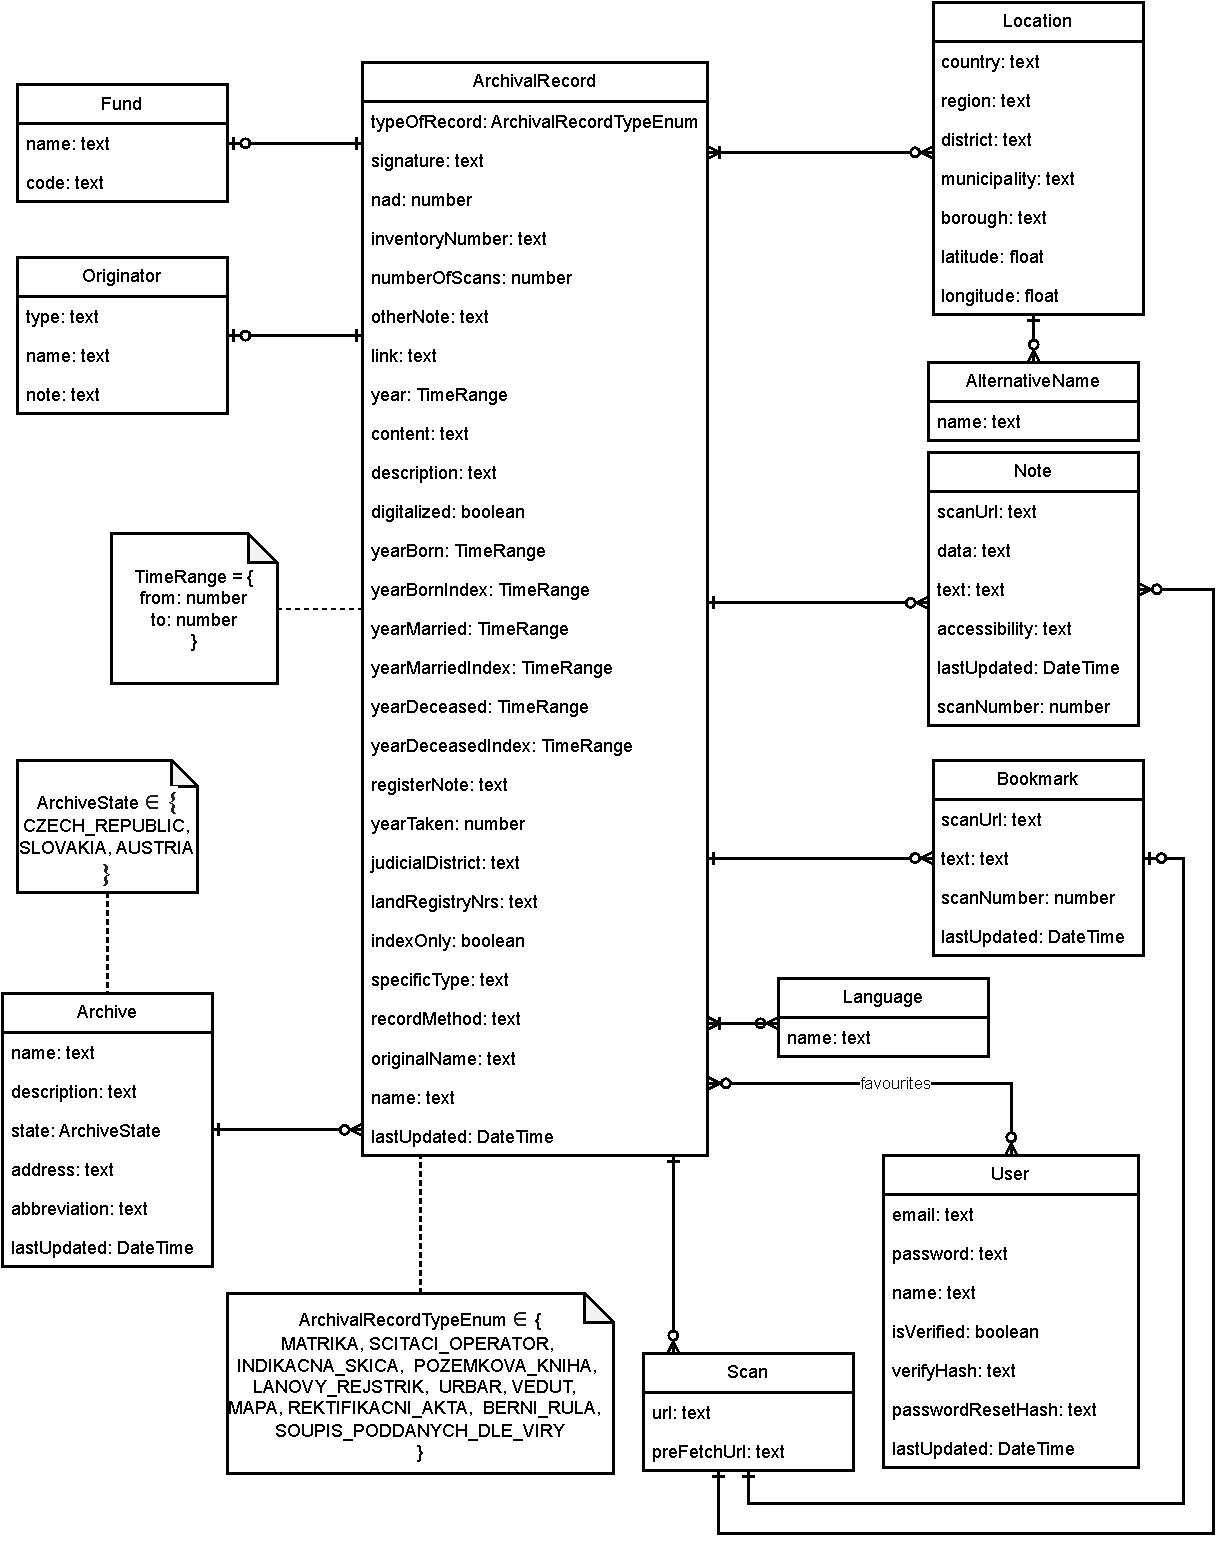
\includegraphics[scale=.75]{obrazky-figures/specification/domain_model.pdf}
        \caption{Doménový model}
\end{figure}

\newpage
\section{Použitá architektura a~technologie}
U této aplikace se neočekává velká zátěž ze strany uživatelů, takže použití distribuované architektury pro aplikační server by zde bylo kontraproduktivní a~pouze by vedlo ke zvýšení režie a~nákladů na provoz samotného systému. Jako vhodná se zde jeví monolitická architektura se~třemi logickými vrstvami a~separátní klientskou aplikací. Tato práce se primárně věnuje návrhu čistě klientské aplikaci. U~aplikace se očekává vyšší míra čtení než zápisů. Jelikož je v~plánu implementovat fulltextové vyhledávání, tak je zvolen návrhový vzor CQRS \cite{cqrsMicrosoft, cqrsAws}, kde dochází k~synchronizaci relační databáze s~nerelační. Tato kombinace umožňuje využívat výhody obou typů databází. V~rámci serverových technologií dojde k~omezení na striktně typované, jelikož dynamické typování v~rámci většího projektu je spíše kontraproduktivní a~zatemňuje kód. Z~analýzy aktuálně používaných systémů je patrné, že většina z~nich běží na Javě. V~tomto případě bude využit aplikační rámec Spring boot \cite{springBoot}, který je postaven na programovacím jazyku Java. Java splňuje všechny podmínky, mezi které patří silné typování, bohatý ekosystém, multiplatformita a~opensource. Mezi technologiemi pro vývoj klientských aplikací nemá smysl uvažovat něco jiného než reaktivní JavasSriptový aplikační rámec. Z~jednotlivých aplikačních rámců byl zvolen React.JS \cite{reactDev} pro jeho vhodnou modulárnost vzhledem k~velikosti projektu. JavaScriptový aplikační rámec je rozšířen o~Typescript \cite{typescript}, čímž je docíleno statického typování. Pro centralizované ukládání a~přístup k~datům je využit state management knihovna Redux \cite{redux}. Tato kombinace umožní vytvořit rozšiřitelnou a~snadno udržitelnou aplikaci, která bude ctít dobré programátorské principy jako SOLID \cite{solid} nebo pravidla čistého kódu.
\newpara
Nyní budou představeny jednotlivé technologie a určité aspekty, na něž bude dále odkazováno v kapitole \ref{chap:implementation} Implementace.

\subsection{Relační databáze}
Relační databáze \cite{relationalDatabaseIbm, relationalDatabaseOracle} ukládá data do tabulek, mezi kterými mohou existovat vztahy pomocí primárních a~cizích klíčů. Každá tabulka obsahuje množinu záznamů, jež mají stejnou strukturu. Každý jednotlivý záznam musí mít jednoznačný identifikátor. Identifikátory umožňují definovat vztahy mezi jednotlivými záznamy i~napříč různými tabulkami. Relační databáze jsou velmi pesimistické a~řádí se mezi silně konzistentní databáze. Jednotlivé operace jsou prováděny v rámci databázových transakcí, které se na konci potvrdí, případně zamítnou. Tímto se eliminuje případ, kdy by nastal výpadek uprostřed operace a~například z~jednoho bankovního účtu by odešly peníze, ale na druhý se již nepřipsaly. Relační databáze splňují \texttt{ACID} vlastnosti, mezi než patří atomicita, konzistence, izolace a~trvanlivost.

\subsection{Databázové indexy}
Databázové indexy \cite{databaseIndexIbm, databaseIndexJimmy, databaseIndexRimon} jsou klíčovou součástí databází, bez nichž by nešlo provádět efektivní vyhledávání a dotazování nad velkými datovými sadami. Každý index má specifikovaný sloupec, podle kterého je seřazen, a~následně se díky němu zvyšuje rychlost vyhledání záznamů, jež splňují konkrétní podmínky. Implicitně databáze vytváří indexy pro primární klíče.
\newpara
Existují dva hlavní typy databázových indexů, B-stromové indexy a~hashovací indexy. B\mbox{-strom} je vyvážená datová struktura, kde uzly obsahují indexované klíče. Každý uzel má určitý počet klíčů. Celá struktura je seřazená, klíče s nižší hodnotou se nachází vlevo a~s~vyšší vpravo. Použití seřazeného B-stromu posune vyhledávání z~třídy lineární časové složitosti do třídy logaritmické, přičemž tato časová složitost je garantována díky vyvažování B-stromu.

\begin{figure}[htbp]
    \centering
        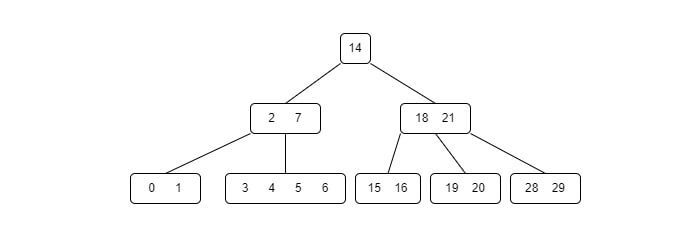
\includegraphics[scale=.6]{obrazky-figures/implementation/b_trees.jpg}
        \caption{Vizualizace B-stromu\protect\footnotemark}
\end{figure}
\footnotetext{\href{https://www.tutorialspoint.com/data_structures_algorithms/images/b_trees.jpg}{https://www.tutorialspoint.com/data\_structures\_algorithms/images/b\_trees.jpg}}



\newpage
\noindent
Alternativou k B\mbox{-stromům} jsou hashovací indexy \cite{hashTableYourBasic}, které využívají hashovací funkci. Funkce transformuje klíč na index v tabulce. Použitím tohoto přístupu se dosáhne konstantní časové složitosti, a to za předpokladu, že je zvolena vhodná hashovací funkce, jež klíče distribuuje rovnoměrně, čímž nedochází k častým kolizím klíčů. 

\begin{figure}[htbp]
    \centering
        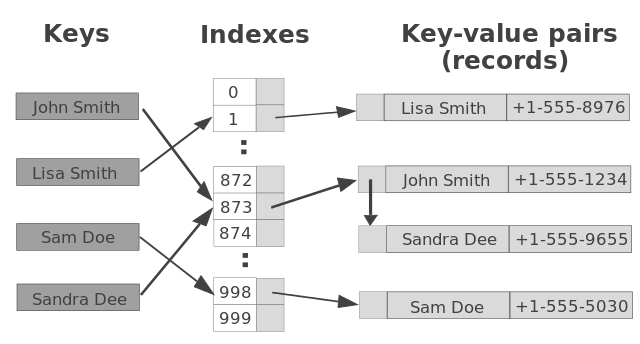
\includegraphics[scale=.65]{obrazky-figures/implementation/hash-table.png}
        \caption{Vizualizace hashovací tabulky\protect\footnotemark}
\end{figure}
\footnotetext{\href{https://yourbasic.org/algorithms/hash-table.png}{https://yourbasic.org/algorithms/hash-table.png}}

\noindent
Databázový index nemusí být pouze pro jeden sloupec, ale může se jednat o index složený, který lze využít v případě, že dotaz obsahuje filtrování na základě více klíčů současně.
\newpara
Použití databázových indexů s sebou nese jistou režii, jelikož tyto indexační struktury zvyšují paměťové nároky a zpomalují operace modifikující data. Při každé operaci, která modifikuje obsah databáze, se musí upravit všechny indexy, jež jsou na daný záznam navázány. Databázové indexy by byly bezcenné v případě, že by nebyly synchronizovány s daty v databázi.

\paragraph{Formální popis relačního datového modelu}\mbox{}\\
\noindent Relační databáze vychází z relačního datového modelu, takže relační databázi lze formálně popsat. Relační datový model je založen na konceptu relační algebry a teorie množin. Každou databázi lze potom chápat jako množinu tabulek.
\[DB = \{T_1, T_2, ..., T_n\}\]
Každá tabulka je definována pomocí matematické relace, která je podmnožinou kartézského součinu jednotlivých domén hodnot. Doména je množina možných hodnot pro daný atribut relace. Databázová tabulka je následně vizuální reprezentací dané relace.
\[R \subseteq D_1 \times D_2 \times \ldots \times D_m\]
Následně je možné použít relační algebru, která nám poskytuje formální operace pro manipulaci s relacemi. Mezi základní operace patří selekce, projekce, sjednocení, rozdíl a kartézský součin.



\subsection{Plné textové vyhledávání}
Plné textové vyhledávání \cite{fullTextSearchMongo, fullTextJosh} je proces hledání a~získávání relevantních informací z~textových dat. Oproti klasickému hledání podřetězce může zvládat hledání synonym, typografickou chybu v~hledaném výrazu nebo hledání podle kořene slova.
\newpara
Kritickou součástí, aby vyhledávání fungovalo podle očekávání, je správné nastavení analyzátorů. Analyzátory v~rámci zpracování textu rozdělují textová data na podřetězce, jež jsou nazývány tokeny. Analyzátory mohou rozdělovat tokeny například pomocí bílých znaků a~interpunkčních znamének. Dalším zajímavým příkladem tokenizeru je Ngram, který rozdělí text na podřetězce do určité délky, což umožňuje vytvořit index pro prefixové a~infixové vyhledávání. Tokeny se následně normalizují, filtrují a~případně se aplikují další transformace. Filtrování probíhá zpravidla na stop slovech, což jsou slova v~daném jazyce mající vysokou frekvenci výskytu v~textu a~nejsou proto relevantní pro vyhledávání. Typickým příkladem stop slov jsou například předložky. Mezi typické příklady normalizérů patří převod na malá písmena, ASCII folding, stemmer a~normalizér synonym. ASCII folding zahrnuje odstranění speciálních znaků, stemmer se stará o~převod slova do základního tvaru a~normalizér synonym převádí synonyma na jednotný tvar. Pro správné fungování musí být nastaven cílový jazyk.


\subsection{Nerelační databáze Elasticsearch}
Elasticsearch \cite{elasticsearch} je distribuovaná, open-source, plně textová vyhledávací a analytická databáze. Databáze vychází z Apache Lucene a je navržena pro zpracovávání velkých dat. Data jsou namísto v tabulkách ukládána v kolekcích JSON dokumentů. Primárním důvodem, proč je tato databáze použita v tomto systému, je podpora plně textového vyhledávání. Databáze pro komunikaci se serverovou částí aplikace nabízí REST rozhraní.
\newpara
V rámci Elasticsearch se rozlišují tři základní typy položek. Jedná se o~Klíčové pole, Plně textové pole a~Obecné pole. Klíčové pole slouží pro ukládání hodnot nevyžadujících analýzu, nebo v případě, kdy je požadováno porovnání na shodu. Klíčové pole je využito u~parametrů, podle kterých jsou záznamy filtrovány. Plně textové pole je využito na položky jako popis archiválie, kde se očekává vyhledávání v~textu. Obecné pole je kombinací dvou výše zmíněných a umožňuje filtrování na přesnou shodu i~vyhledávání v textu.
\newpara
Entity je potřeba obohatit o dodatečné anotace pro použití s Elasticsearch. Díky anotaci \texttt{@Indexed} je povoleno indexování dané entity do Elasticsearch databáze. Následně se musí specifikovat pro jednotlivé atributy, zda se jedná o klíčové slovo nebo plné textové vyhledávání. Pro složitější datové typy se musí vytvořit konvertory zabezpečující mapování mezi objekty v Javě a datovými typy v Elasticsearch. Pro každý atribut, který je anotován plným textovým vyhledáváním, se nastaví analyzátor a pro klíčové slovo normalizer. Je definován normalizer Czech, v rámci něhož je aplikován převod na malá písmena pomocí filtru lowercase a odstranění speciálních symbolů pomocí asciifoldingu. Stejnojmenný analyzátor využívá standardní tokenizér a následně aplikuje filtry: lowercase, czech\_stemmer, asciifolding, czech\_grammar\_normalizer. Token se tedy převede na malá písmena, slovo se analyzuje a převede se do kořenového tvaru. Následně se odstraní speciální znaky a aplikuje se normalizace asimilovaných hlásek. Hlásková asimilace \cite{hlaskovaAsimilace} je jev ve fonetice spočívající ve výslovnostním přizpůsobováním hlásek. V českém jazyce se většinou jedná o asimilaci kontaktní, kdy se přizpůsobují hlásky sousedící.


\section{Tvorba interaktivního prototypu}
\label{sec:funkcni-prototyp}
Před samotným návrhem aplikace a~tvorbou grafického prototypu byl označen za nejkritičtější část systému samotný prohlížeč archiválií, tudíž byly zkoušeny možnosti zobrazení dlaždicových snímků, hledány vhodné knihovny, případně navržena vlastní řešení některých funkcionalit, aby bylo ověřeno, že systém je podle aktuálních požadavků možné realizovat. Prototyp byl realizován v~technologiích, které byly zvoleny pro finální implementaci.

\begin{figure}[htbp]
\centering
    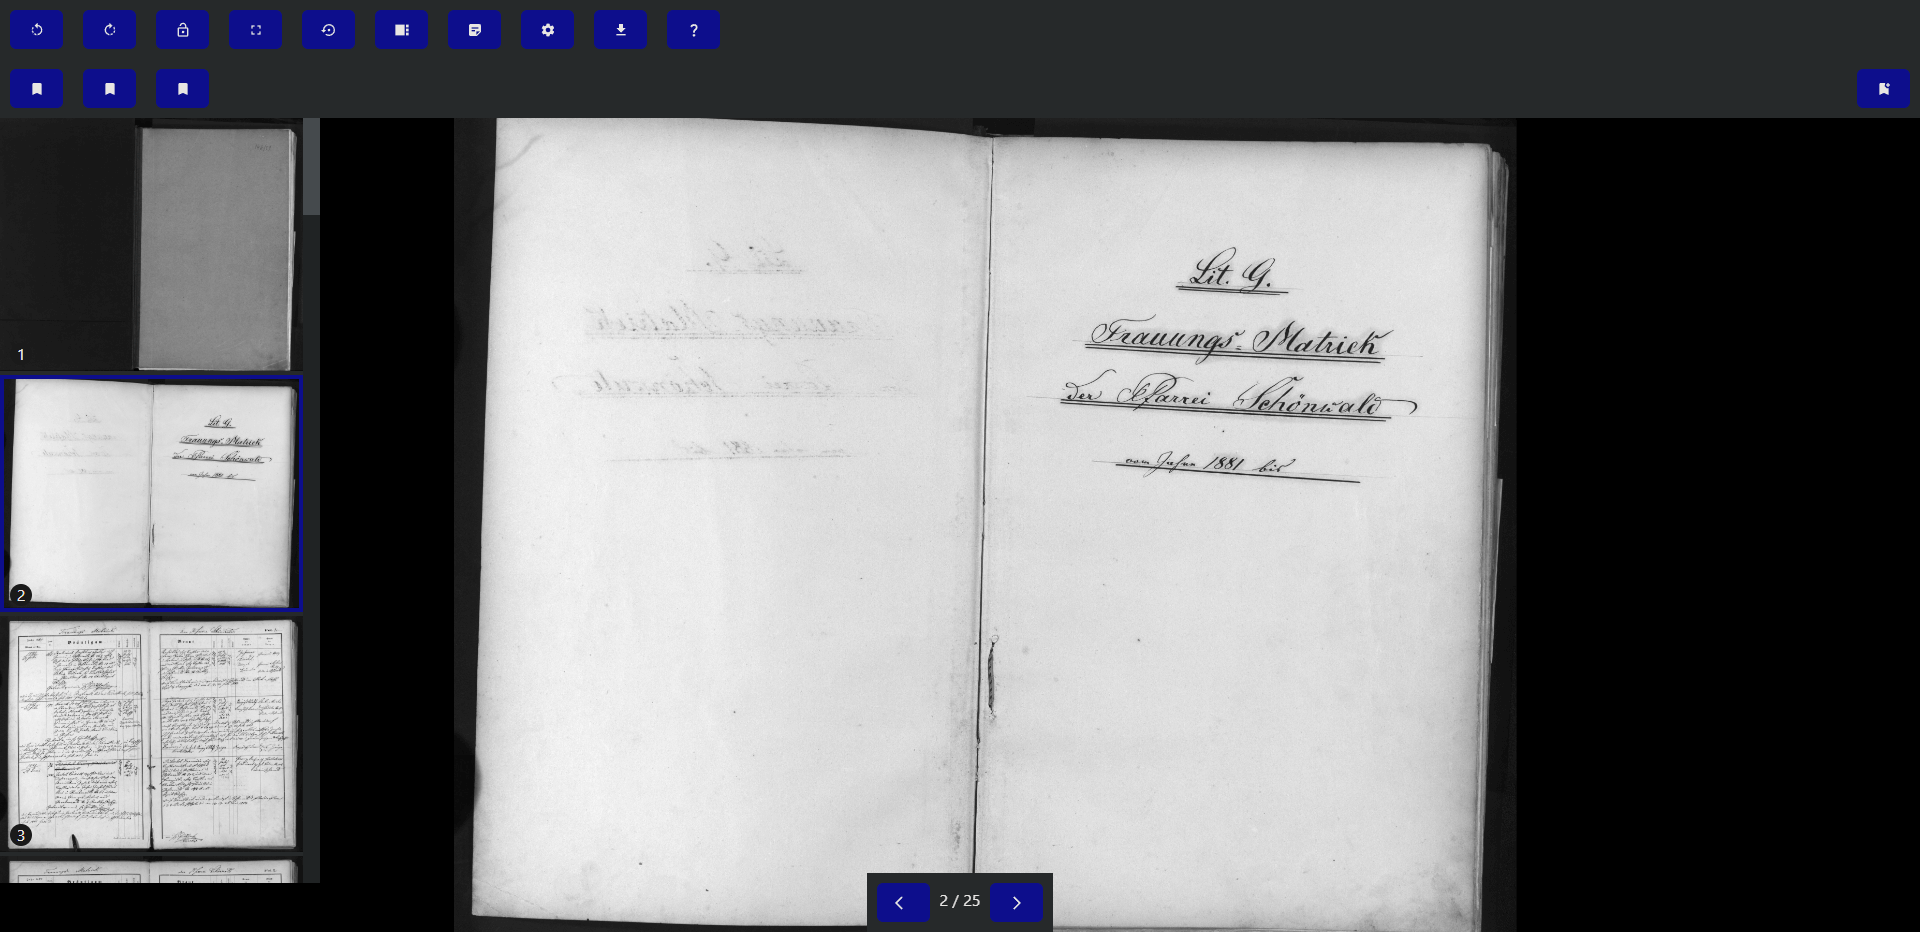
\includegraphics[scale=.2]{obrazky-figures/design/prototype.png}
    \caption{Screenshot z~prototypu}
\end{figure}

\noindent
Experimentálně bylo vyzkoušeno více různých řešení a~vybráno bylo takové, které nejvíce vyhovovalo požadavkům. Jednalo se o~knihovnu OpenSeaDragon podporující jak zobrazování standardních snímků, tak i~snímků využívajících dlaždicové formáty. Knihovna dále obsahuje bohatou sadu funkcí, jež bude stačit rozšířit.